\chapter{Introduction}\label{chp:chp1}

%\begin{flushright}
%  {\em QUOTE GOES HERE }\\
%
%\ \
%
%\normalsize
%{AUTHOR}  
%\end{flushright}


\noindent{Should you choose to seek out one of my friends and ask them about my whereabouts in recent months,
%acquaintances and to enquire of them my whereabouts in recent months
 %they would likely stare at you blankly.  Upon further interrogation 
 they would probably yield the information that I had been noticeable by my absence because I was preoccupied writing about dust, a fact which I imagine they  find bemusing and possibly somewhat concerning.  Blissful as they are in their ignorance of dust (astronomers find no such peace), they do not know the importance of this all-pervading substance.}

The universe is an extremely dusty place.  The ubiquity of dust throughout almost all epochs and environments demands a comprehensive understanding of its formation and evolution, properties and effects.  It plays numerous roles in a variety of scenes; it is a building block of  all solid bodies, a birthing place for molecules, a crucial ingredient in star formation and an extreme annoyance for cosmologists.  It is both a product of physical processes and an agent of chemical ones.

It is perhaps confusing therefore that there is comparatively little consensus regarding the formation processes and natal environments that result in the evolution of certain atoms and molecules into the grains we call dust.  Over the years since the first discovery  of dust in the very early universe, a growing population of astronomers and astrophysicists have turned their attention to the study of dust formation in core-collapse supernovae (CCSNe), in the hope that these objects might prove to be the missing piece of the puzzle.  Recent observations of a number of CCSNe and supernova remnants (SNRs) have lent weight to this theory, with models and analyses of spectral energy distributions (SEDs)  suggesting the presence of large reservoirs of cool, ejecta-condensed dust. 

I have sought to make my own small contribution to this field by exploiting a different observational signature, that of  blue-shifted line profile asymmetries observed in the spectra of many CCSNe and attributed to the formation of dust in the ejecta.  By quantitatively modelling characteristically asymmetric spectral line profiles using a new code, DAMOCLES, I have attempted to determine the rate of dust formation in CCSNe and the expected order of magnitude of the eventual dust masses produced.

Throughout the remainder of this chapter I will attempt to elucidate the above synopsis in more detail.  A brief discussion of the roles that dust plays in the universe will be followed by a summary of our current understanding of dust formation in CCSNe.  I will conclude this chapter with a short justification of the approach that I have adopted for this work and an outline of the structure of this thesis.


\section{A Handful of Dust}


\subsection{A Brief History}

The presence of dust in the universe was first theorised when astronomers observed dark patches of sky in the Milky Way where all of the stars had been ``erased" (see Figure \ref{intro:fig:dustpatch}).  Whilst some claimed that these black regions were in fact a true absence of stars resulting from some anomaly in the stellar distribution, others felt that it was more likely that an obscuring cloud of material was blocking the light from the stars behind.  In 1930, Donald \citeauthor{Trumpler1930} confirmed this latter theory by considering the apparent magnitudes and colours of stars located at different angles to the galactic plane, discovering that those closer to the plane appeared redder than their more distant counterparts.  This was the first evidence of interstellar reddening and the beginnings of our understanding of dust as a scatterer, absorber and emitter of radiation.

For the next few decades, dust was thought to be largely an irritating obstacle to observing and comprehending more interesting facets of the universe.  We now have a much fuller understanding of the variety and importance of the roles that dust plays throughout astrophysics.

\begin{figure}
\centering
\includegraphics[scale=0.8]{chapters/chapter1/figs/black_patch_B68.jpg}
\caption{The dark globule Barnard 68, LDN 57.  ESO press release 30 April 1999.}
\label{intro:fig:dustpatch}
\end{figure}

\subsection{The Roles of Dust in the Universe}

Despite comprising only $\sim$1\% of the mass of the interstellar medium (ISM), dust grains account for as much as 30\% of the total galactic luminosity via their emission in the infra-red (IR) \citep{Li2003}.  In the cycle of matter from the ISM to condensing clouds to stars and back again, dust is far more than a passive passenger along for the ride.  Whilst residing in the ISM, dust is important in determining its thermodynamics.  It acts both as a heating agent via the emission of photoelectrons in regions of strong ultra-violet (UV) radiation and a coolant in dense regions via the emission of IR radiation.  In this role as a coolant, dust is also crucial to the process of star-formation, helping to remove gravitational energy and allowing the natal cloud to collapse.  Dust also contributes to the star formation process by shielding the gas from ionising radiation, helping to speed up the construction of the protostellar core. 

In addition to the above physical functions, dust plays an essential part in chemical processes.  Heavy elements in the local medium are depleted through their inclusion in dust grains.  These grains  attract gaseous atoms to their surfaces and catalyse the formation of molecules which are then released back into the surrounding medium.

Dust does not reside solely in the ISM however.  It is present in  large quantities in the circumnuclear tori found around active galactic nuclei.  Dust is also found between planets, around stars and in protoplanetary discs, where dust grains constitute the smallest unit of the building blocks that will go on to form planetesimals and planets.  These grains may even be responsible for the origins of life.  

The more detailed our understanding of dust as an astrophysical community, the more accurate we can make our inferences across an entire range of  fields.  There is arguably no other topic in astronomy that has such wide-ranging effects.


\subsection{The Medium of Dust}

\subsubsection{Composition}

An increasingly detailed knowledge of the nature and properties of dust has developed over the last few decades. Dust grains have their terrestrial analogue in soot or very fine sand rather than in the dust bunnies that one may find behind the sofa.  When found in the ISM they are generally small, between 0.05\micron\ and 0.25\micron\ in radius, and are normally predominantly composed of carbon or silicates.  Carbonaceous grains may take many forms ranging from structured solids such as diamond and graphite to amorphous molecules and aromatics.  They are generally found to be strongly attentuating.  Silicates tend to be more glassy and contain silicon and oxygen potentially with the dirtying addition of magnesium, iron or other heavier elements.  Condensates of more complex molecules such as olivine (MgFeSiO$_4$) and pyroxene (MgSiO$_3$) make up these grains.  

\subsubsection{Optical Properties}
\label{opt_prop}
Whilst an increasingly strong picture of the composition and properties of dust is becoming apparent, there are still a number of largely unresolved issues regarding the makeup of a dusty medium.
Different species and composites thereof have different optical properties.  In order to model the absorption and scattering of radiation off dust grains it is necessary to first know the complex refractive indices of a given species over the relevant wavelength range (see Section \ref{scn:mie_theory}).  Laboratory measurements have produced a number of different sets of optical constants for a variety of carbonaceous and silicate species and these are well-utilised throughout the field.  It is noted at this early juncture however that in many cases there are numerous, somewhat contradictory, sets of optical constants for a given species and that these variations can potentially cause a degree of confusion regarding the results of models that use them (e.g. \citet{Owen2015}).  
%This topic will be discussed in detail later in this thesis (SECTION).

\subsubsection{Dust Grain Morphology}

Dust grains are generally assumed to be spherical in order to make their simulative treatment more straightforward but in reality dust shapes are actually much more complex.  Sophisticated models of dust grains sometimes adopt a continuous distribution of ellipsoids to represent dust grain shape.  This allows grains to take any ellipsoidal form ranging from flat discs to needles to perfect spheres.  However, even this more detailed consideration omits structures that are akin to long strings or to fluffy particles (not dissimilar to a tumble dryer ball in shape). Heretofore, the vast majority of models, including DAMOCLES, have only considered spherical grains and this wide variety of shapes therefore represents a significant modelling challenge to be addressed in the future.

Dust in the universe follows a cycle.  From its stellar birthplace, it is ejected and slowly integrates itself with the ISM before condensing into molecular clouds and ultimately once again returning to stars.  Most of the knowledge of the properties of dust applies only to grains in the ISM, which are found to follow a grain radius distribution $n(a) \propto a^{-3.5}$ as described by \citeauthor{Mathis1977} in 1977.  This distribution does not necessarily apply immediately after their formation, however, as grains are subject to numerous forces that can result in their destruction, sputtering or evaporation.  The grain size distribution and relative abundances of species of newly-formed grains are still topics in dispute and are issues that I attempt to address in my models.  The issue of dust grain shape will hopefully be addressed in future versions of DAMOCLES (see Section \ref{limitations}).


\subsection{Origins of Dust in the Universe}
In an effort to explicate the motivations behind studying dust, I have so far mostly limited my discussion to the evolution and properties of dust after the initial stages of its formation.  The most current and contentious debate, however, is over the natal environment of dust grains.  

Over the past two decades, several high redshift galaxies and quasars (QSOs) have been found to contain significant masses of dust as evidenced by the detection of red-shifted dust emission at sub-millimetre wavelengths \citep{Carilli2001, Omont2001, Bertoldi2002, Bertoldi2003, Watson2015}.  Warm dust masses ($T\sim50K$) inferred from these observations are of the order of $10^8M_{\odot}$ at very early epochs $z \gtrsim 6$ \citep{Robson2004,Beelen2006,Dwek2007}.  A dusty, evolved galaxy has even been found to have existed during the epoch of reionization at $z=7.5$ when the universe was only about 500 Myr old \citep{Watson2015}.  The presence of such large quantities of dust at such an early stage of the universe's evolution presents a significant challenge to astronomers to find a source.  

Until these recent observations, Asymptotic Giant Branch (AGB) stars were thought to be the dominant source of dust in the universe.  AGB stars are evolved stars with stellar masses in the range $0.85M_{\odot} \lesssim M_{*} \lesssim 8M_{\odot}$.  These stars have reached a stage of evolution that is characterised by separate shells of hydrogen and helium burning surrounding a dense carbon-oxygen core. They are extremely luminous ($>10^3L_{\odot}$) and have strong winds that can cause the star to lose up to 70\% of its mass resulting in the formation of an extended circumstellar envelope \citep{Wood2004a}.  It is in these regions that conditions are thought to be appropriate for dust formation and this process has been studied in the environment of AGB stars by many authors (e.g. \citet{Gail1999,Cherchneff2000,Ferrarotti2005}.  The theory has been confirmed on numerous occassions by observations of dust  in these objects \citep{Meixner2006,Matsuura2009,Sloan2009,Boyer2011,Boyer2012,Riebel2012,Matsuura2013}. Theoretically, AGB stars may be capable of producing as much as ~0.04M$_{\odot}$ of dust for a narrow range of stellar masses around 4M$_{\odot}$ \citep{Ferrarotti2006}.  For a wider range of progenitor masses they are predicted to produce a typical dust mass of 0.001M$_{\odot}$. However, it is unlikely that enough low-intermediate mass stars, which take around 0.1-10Gyr to reach the AGB \citep{Salaris2014} and likely formed around $z\lesssim20$ with the star formation rate (SFR) peaking at $z\sim5$ \citep{Greif2006}, had enough time to reach the AGB stage of their evolution.  The few higher mass stars that may have done likely cannot have contributed significantly to the large dust masses seen at very early epochs.  In addition to this, local metal-poor galaxies contain more dust than can be accounted for by dust formation in AGB stars alone.  In fact, it has been shown that AGB stars are likely to contribute only about 1.6\% of the $2\times 10^8M_{\odot}$ of dust observed in the galaxy J114816.64+5251 at $z=6.4$ \citep{Dwek2007,Matsuura2009,Matsuura2013}.  Such evidence has been used to rule out the possibility that AGB stars could account for the dust masses observed in the early universe \citep{Michalowski2015}.

CCSNe are one of the few potential sources that could contribute large quantities of dust at early epochs.  With the probable elimination of the theory that AGB stars were a significant source of dust at high redshifts, attention is now strongly focussed on determining whether dust formation in CCSNe could resolve the dust mass dilemma both at high redshifts and in local galaxies.

\begin{figure}
\centering
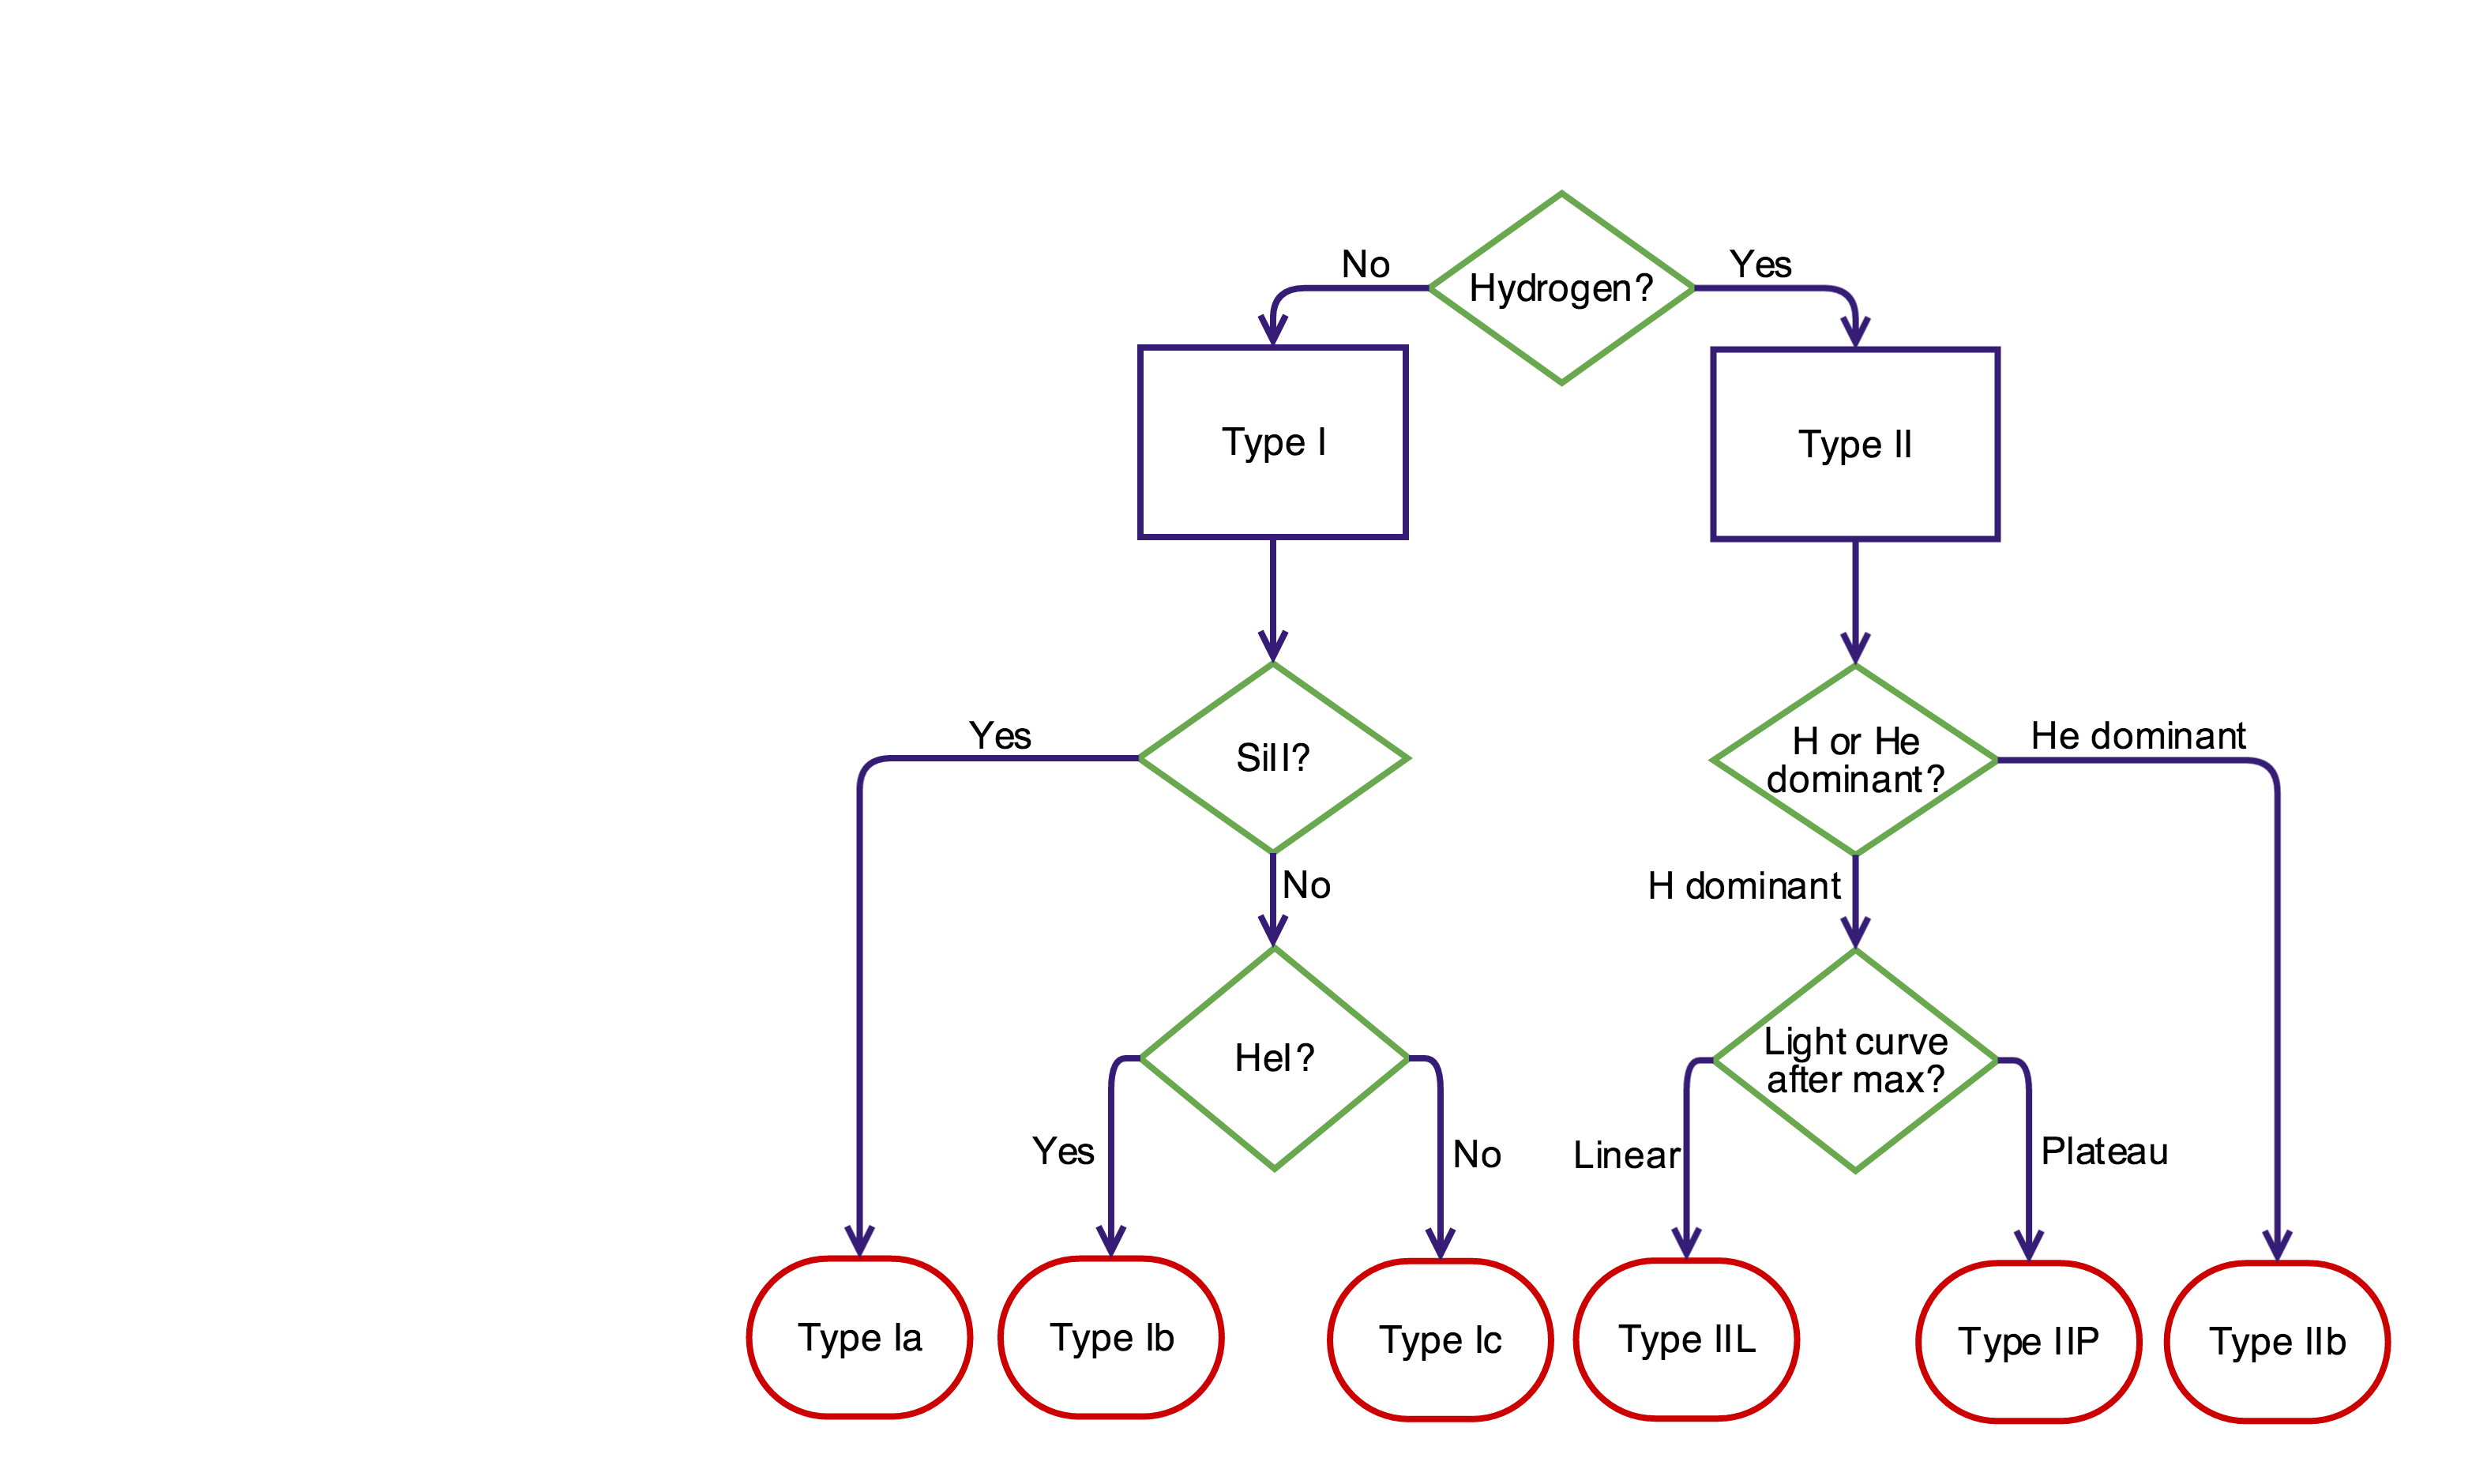
\includegraphics[clip=true, scale = 0.2, trim= 930 50 55 210]{chapters/chapter1/figs/sn_classification.png}
\caption{A flowchart summarising the supernova classification scheme}
\label{intro:fig:sn_class}
\end{figure}

\section{Core-Collapse Supernovae as Dust Factories}

Supernovae are the violent explosions that are the death of stars.  They evolve very quickly and create extreme conditions.  Focus on supernovae as a possible source of dust in the universe has been motivated by the physical conditions that they produce shortly after their outbreak and by the presence of large quantities of heavy elements that constitute the integrant ingredients of dust grains.

% are thought to be a possible source of dust in the universe since they produce large quantities of heavy elements and have physical conditions that are potentially suitable for the growth of dust grains.  



\subsection{Types of Supernovae}

Supernovae may be classified into a number of different types.  They are bisected initially into Types I and II according respectively to the absence or presence of hydrogen in their early spectra.  Further sub-classifications depend on  other features in the early spectra, properties of later spectra and the evolution of the  light curve after maximum light.  A summary of the supernova classification scheme is presented in Figure \ref{intro:fig:sn_class}.  



If the initial classification is Type I then all further sub-classifications depend solely on the properties of the early spectra (a few days after explosion) as detailed in Figure \ref{intro:fig:sn_class}.  Type II supernovae are somewhat more complex in their categorisation.  After classification as a Type II, further subdivisions depend on the dominance of hydrogen or helium in \textit{later} spectra.  Helium dominant supernovae are classified as Type IIb and hydrogen dominant supernovae are classified as either Type IIL (those which have a linearly decaying light curve after maximum light) or Type IIP (those that exhibit a plateauing light curve after maximum light).  Type IIn supernovae are omitted from the summary presented in Figure \ref{intro:fig:sn_class} as they cannot be classified straightforwardly via a bifurcating process.  Type IIn supernovae will generally have strong emission lines, particularly hydrogen lines, often with complex profiles.  Crucially, the spectra of Type IIn supernovae do not exhibit the broad absorption features frequently seen in other types and instead contain narrow lines (hence Type IIn).  

\begin{figure}
\centering
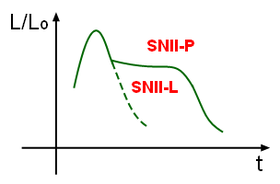
\includegraphics[clip=true, scale = 1, trim=0 0 0 0]{chapters/chapter1/figs/light_curves.png}
\caption{Illustration of the different shapes of light curves for Type IIP and Type IIL supernovae.}
\label{fig:light_curves}
\end{figure}

\subsection{From Massive Stars to Remnants}

It is generally accepted that the progenitors of Type Ia supernovae are white dwarfs that exist in a binary system with another star \citep{Wang2012}.  The accretion of material from one star to another results in a thermonuclear explosion, a mechanism that is unique to Type Ia supernovae.  There have not been any observations suggestive of ejecta-condensed dust forming in the aftermath of a Type Ia supernova and I therefore do not consider these objects any further, focusing my attention solely on supernovae that explode via the core-collapse mechanism.  

Broadly, this process is initiated when a massive star ($\ge 8$\msun) starts to fuse heavier elements. The fusion of ever heavier elements generates increasingly less energy whilst also causing the mass of the core to increase.  Eventually, radiation pressure drops sufficiently that the core can no longer support itself against its own self-gravity and begins to collapse rapidly. Within milliseconds, the core reaches extremely high densities and, when it can no longer condense further, ``bounces" off itself causing  an immense shockwave to propagate outwards and a vast quantity of energy to be released via the expulsion of neutrinos.  Much of this complex process is still poorly understood and interesting models are currently being produced recreating these very early stages using a numerical approach \citep{Hammer2010,Takiwaki2014,Wongwathanarat2015}.  Though the explosion mechanisms of CCSNe are largely beyond the scope of my work, some attention will be paid to these models later in this thesis since instabilities that arise in these early stages can influence the structure of the ejecta at later stages of its evolution.

For many years after the explosion, the supernova (now a remnant) is in the free-expansion phase \citep{Landau1959,Ostriker1988}. During this phase, the mass and velocity of the expanding supernova massively exceed those of the surrounding medium, fortuitously allowing the behaviour of the SNR to be analysed as if it were expanding into a vacuum.  The shock radius during this phase may therefore be calculated simply as $R_s = v_s t$.  As the shockwave propagates through the ISM, interstellar material that has been compressed by the forward shock begins to accumulate.  At the same time a reverse shock wave begins to propagate back through the ejecta.  It is during this phase, which arises very soon after the initial explosion and typically lasts for a few hundred years, that the physical conditions in the ejecta are thought to be optimal for dust formation.  The phase ends when the mass of material ahead of the forward shock is of a similar magnitude to that behind and the mathematical treatment of its behaviour must be altered as it enters the Sedov-Taylor phase.
 
 \subsection{Energetics in Core-Collapse Supernovae}

Energy of sn ejecta and the formation of emission lines.  Freeze-out. IR catastrophe?

Include e.g. Balmer line chart


\subsection{Dust Formation and Destruction in CCSNe}
%in CCSNe?  See osterbrock.
\label{scn:dust_formation}
The formation of dust was originally thought to result from the stochastic process of classical nucleation whereby particles coalesce to form the seeds of dust grains.  These seeds become the nucleation sites from which grains are ultimately born through the aggregation of further particles.  Various models of dust formation in the ejecta of CCSNe have used this approach \citep{Kozasa1989, Todini2001,Nozawa2003, Schneider2004}.  

More recently, several models of dust formation in CCSNe that consider the effects of chemistry on the growth of dust grains have been published.   These models consider the chemical composition of the gas and include chemical reaction rates thereby considering the manner in which molecular evolution influences dust grain formation and growth rates \citep{Cherchneff2009, Cherchneff2010, Sarangi2013, Sarangi2015}.

Models using both methods have predicted dust masses of the order of 0.1-1\msun of dust forming within the ejecta of CCSNe of progenitor masses between 12-40\msun within the first few years after the initial explosion.

%Talk more here about the quantities via each method - see Gomez review

\subsection{The Three Signatures of Dust}
\label{three_sigs}

%POLARISATION = four.  Should include and also include reference to gomez review 2013.

The presence of dust in the ejecta of CCSNe can be indicated by three main signatures: 

\subsubsection{A decrease in the light curve} 
As the dust begins to form in the ejecta, UV and optical light is absorbed by the dust causing a decrease in the light curve at these wavelengths.

\subsubsection{Excess IR emission}
An increase in emission in the IR occurs contemporaneously with the decrease in the UV-optical light curve.  A thermal MIR excess is caused by warm dust and an excess in the far-IR and sub-mm is the result of cold dust.  The increase in emission in these wavelength can be caused by newly-formed dust condensing in the ejecta but can also be a result of the illumination of pre-existing dust

\subsubsection{Blue-shifted line profiles}
Finally, the onset of the formation of dust can cause an asymmetry in line profiles in the optical and IR.  The absorption and scattering of optical or near-IR radiation by newly-formed dust within the ejecta can result in an asymmetry between the red and blue shifted components, with redwards 
emission from the far side of the ejecta undergoing greater absorption and resulting an overall shift of the profile to the blue.
\\

\noindent All three of these signatures have been discussed in detail over the timeline of this subject but the focus has been on using the excess IR emission seen in the SED of CCSNe to determine quantitatively dust masses in these objects.  This approach has resulted in a lively debate regarding the quantities of dust that CCSNe are capable of producing.
 
 \subsection{Observing Dust}

Add more here about observing dust continuum emission in the IR.  Then move onto line profiles.

Numerous telescopes have recorded spectra of CCSNe in the optical and IR, some with extremely high resolution.  The Anglo-Australian Telescope (AAT), the Cerro Tololo Inter-American Observatory (CTIO), the Hubble Space Telescope (HST) and the Very Large Telescope (VLT) have all observed several supernovae in the optical including SN 1987A.  Other telescopes such as  the two Gemini Multi-Object Spectrographs (GMOS) have also taken spectra of numerous CCSNe.

Advances in digital storage have allowed for spectral and photometric observations to be made easily available online.  Many observatories now publish their recent observations online in archives and are working to upload observations that pre-date file sharing services.  Much of the data used in this thesis was obtained from these archives.


\subsection{The Dust Mass Debate}

The formation of dust grains requires densities high enough for interaction between particles to take place, but temperatures that are cool enough to allow the grains to form and survive.  The theory that the ejecta of a CCSN in its free-expansion phase could provide these conditions  was first hypothesised by \citeauthor{Cernuschi1967} in 1967 and they have now long been thought to be potential dust factories \citep{Hoyle1970, Kozasa1991, Todini2001,Nozawa2003}.  The ejecta cools rapidly as it expands and there is an abundance of heavy elements.  In order to account for the large masses of dust seen in the early universe, it is estimated that CCSNe would need to produce  0.1-1.0~M$_\odot$ of dust per CCSN  \citep{Morgan2003, Dwek2007}

Until recently, supernovae had been largely dismissed as a significant source of dust.  Observations over the last decade at mid-infrared (MIR) wavelengths of warm dust (200 - 450K) emission from CCSNe has suggested that the quantities of ejecta-condensed dust produced during the first 1000 days were typically $\leq$ 10$^{-3}$~M$_\odot$  \citep{Sugerman2006, Meikle2007, Kotak2009, Andrews2010, Fabbri2011}.  This is much less than theoretical models predict (see Section \ref{scn:dust_formation}) and would not account for the dust masses observed in the early universe.  These observations indicated the need to find another early-time source of dust.

\subsubsection{Cassiopeia A}

In 2003, however, the field was shaken by the report that 2-4M$_{\odot}$ of cold dust (20K) had been detected via sub-mm emission in the 300-year old SNR Cassiopeia A (Cas A) using SCUBA \citep{Dunne2003}.   A heated debate followed as astronomers contested the source of the observed dust.  \citet{Dunne2003} had concluded that the dust was associated with the remnant based on the high spatial correlation of the sub-mm emission from the cold dust and the forward and reverse shocks that were traced via X-rays. \citet{Krause2004} refuted this suggestion using analyses of the line emission and absorption to conclude that the dust was in fact located in clouds along the line of sight to the remnant.  A determination was sought by considering the polarisation of the dust emission.  As discussed in the previous section, the asymmetric nature of expansion likely results in a degree of polarisation relative to stationary dust located in the ISM.  Observations of Cas A in the sub-mm were made using the SCUBA polarimeter and the emission was found to be extremely polarised to a fraction of 30\% (compared to typical ISM fractions of 2-7\%).  A reevaluation of the dust mass based only on the polarised emission still estimated the mass of dust in Cas A to be ~1M$_{\odot}$ \citep{Dunne2009}.

\begin{figure}
\centering
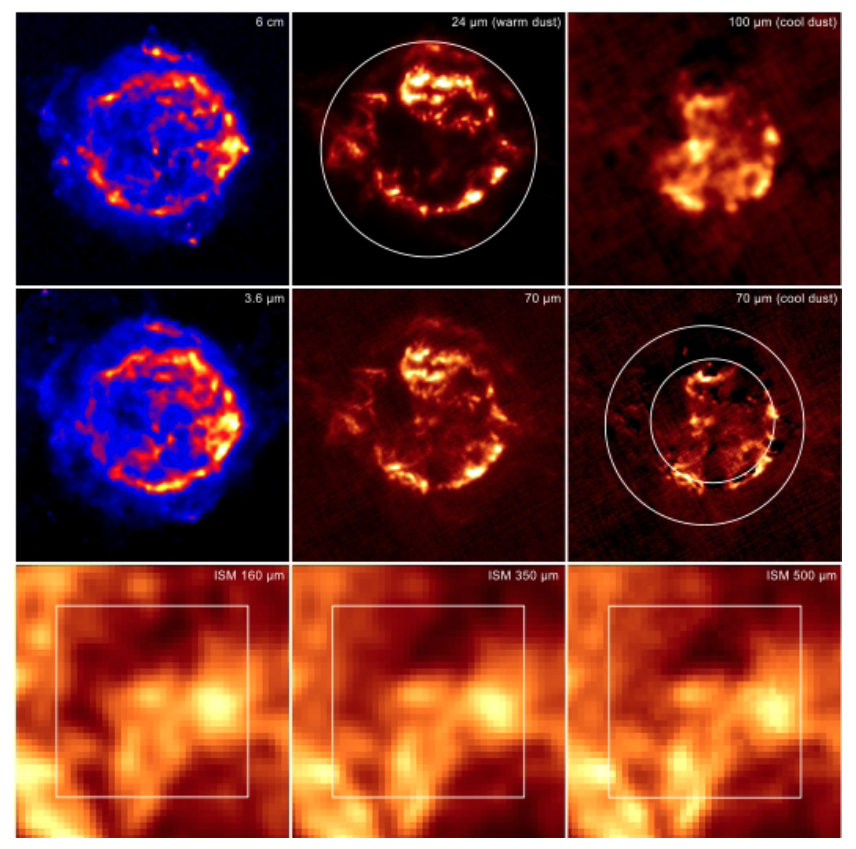
\includegraphics[clip=true,scale=0.425,trim= 0 0 0 0]{chapters/chapter1/figs/CasA.png}
\caption{Images of Cas A at IR, sub-mm and radio wavelengths.  The top six images are 7' on a side and the bottom three are 10' on a side.  The inner and outer circles in the middle-right image correspond to the reverse and forward shocks respectively according to \citep{Gotthelf2001}.  Image taken from \citet{Barlow2010}.}
\label{fig:CasA}
\end{figure}


Even this revised estimate was still uncomfortably large compared to previous estimates.  Sadly, SCUBA was taken offline shortly after this observation and so follow-up observations of Cas A and other remnants was not possible.  It was only with the advent of the \textit{Herschel} mission that the presence of cold dust in SNRs could again be investigated via emission in the sub-mm.  These \textit{Herschel} observations have, somewhat surprisingly for many in the field, consistently revealed dust masses of the order of 0.1-1.0M$_{\odot}$ in a number of SNRs.

%Critical to the investigation of dust formation in SNRs in recent years have been a few key objects, namely Cas A, the Crab nebula and SN~1987A.  As a central focus of this thesis, I will discuss the history of SN~1987A and dust formation within its ejecta in detail at the start of Chapter \ref{chp:chp5} and so I limit my discussion here to just Cas A and the Crab nebula. 

By 2009 large masses of dust had been detected in Cas A using SCUBA.  As the first result of its kind, and with a great many questions left unanswered, it was crucial to establish this result as conclusively as possible.   Observations of Cas A using \textit{Spitzer} detected emission from warm dust between 24$/mu$m - 70$/mu$m analysis of which established a dust temperature of 60 - 120K and a dust mass of 0.02 - 0.054M$_{\odot}$ \citep{Rho2008}.  Subsequent observations using \textit{Herschel} detected a cool dust component of ~0.075M$_{\odot}$ giving a total dust mass in Cas A of ~0.1M$_{\odot}$ \citep{Barlow2010}.  Like many Herschel observations, it is difficult to conclusively determine the location of the dust as within the remnant rather than in clouds in the foreground or background.  Images of Cas A across a range of wavelengths are presented in Figure \ref{fig:CasA}.  

\subsubsection{The Crab Nebula}

The Crab nebula was first detected by Chinese astronomers in 1054.  A pulsar at the heart of the nebula illuminates the surrounding gas and dust and provides a rare opportunity to probe dust masses in a centuries old remnant.  Unlike Cas A, the Crab does not have contaminating clouds of dust in its foreground and background ensuring that any detections of dust from this location are likely to be associated with the remnant.
 
\textit{Spitzer} and \textit{Herschel} observations have been made of this remnant and both have detected dust in the ejecta.  Spitzer, however, only detected $2.4\time10^{-3}$M$_{\odot}$.  Further soectroscopic and photometric observations with Spitzer, Herschel and Planck allowed the full range of the SED to be investigated and allowed for synchortron and line emission to be well-characterised.  Subtracting this from the continuum observations yielded two dust components, a warm component at 63K estimated to have a mass of ~$10^{-3}$ and a cool component at  34K with an estimated mass of 0.1 - 0.2M$_{\odot}$ \citep{Gomez2012,Temim2012}.  As might be expected, the dust is predominantly co-located with the gas in dense filaments (see Figure \ref{fig:Crab}).
 
 These dust masses were based on a two-component dust fitting.  Further analyses and models of these results have resulted in revised estimates of the mass of dust in the Crab nebula.  Multi-component fitting with multiple grain size by \citet{Temim2013} gave rise to a dust estimate of 0.02-0.13M$_{\odot}$, consistent with the lower end of the previous estimate.  However, recent radiative transfer models by \citet{Owen2015} that account for varying grain size distributions, gas geometries and a more realistic heating source derive dust masses consistent with the estimated 0.1-0.2M$_{\odot}$ of \citet{Gomez2012}.  If the dust in the ejecta is assumed to be clumped however, as is likely more realistic, then 0.4 - 0.6M$_{\odot}$ of amorphous carbon grains are required to fit the SED.  At this time, the Crab nebula was the only object to have provided a clean view of large masses of dust ($>10^{-3}$M$_{\odot}$).
 
 \begin{figure}
\centering
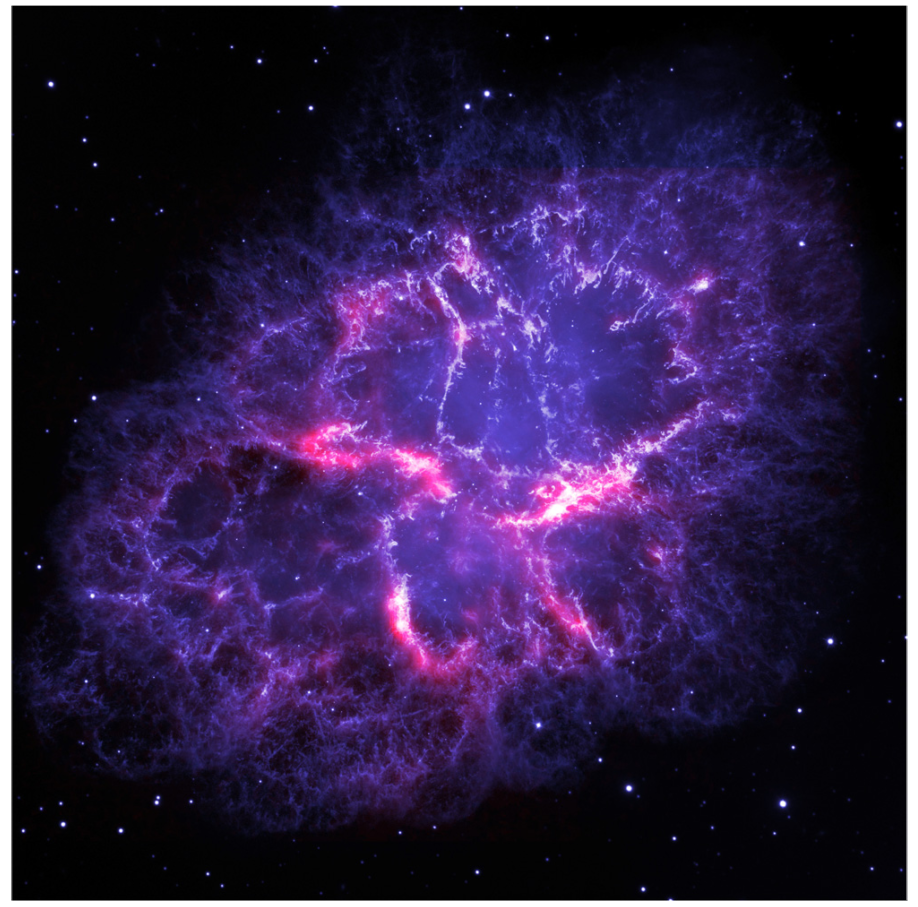
\includegraphics[clip=true,scale=0.3,trim= 0 0 0 0]{chapters/chapter1/figs/Crab.png}
\caption{Composite image of the Crab nebula using Hubble Space Telescope (HST) optical line emission data (blue-white) and {\em Herschel} 70$\mu$m dust emission (red) illustrating the close alignment between the optical knots and filaments.  Credits: Oli Usher (UCL); \textit{Herschel Space Observatory, Hubble Space Telescope}: ESA, NASA.  Image taken from \citet{Owen2015}.}
\label{fig:Crab}
\end{figure}
 
 \subsubsection{SN~1987A}
 
 Perhaps the most critical discovery however, was that of dust in the ejecta of SN~1987A.  This object is uniquely helpful in the study of supernovae due its location only ~50kpc away.  Dust had long been theorised in the ejecta of SN~1987A but only in comparatively small quantities.  Observations of blue-shifted line profiles in the optical and of warm dust emission in the MIR confirmed this hypothesis with dust mass estimates of ~$5-20 \times 10^{-4}$M$_{\odot}$ forming in the first 1000 days\citep{Lucy1989,Roche1989,Bouchet1991,Wooden1993,Ercolano2007}.  In 2010, this view was fundamentally altered by observations by \textit{Herschel} that indicated the presence of 0.4-0.7M$_{\odot}$ of cold dust.  Further observations with Herschel and the Atacama Large Millimetre Array (ALMA) not only confirmed this dust mass estimate but also had sufficient spatial resolution to conclusively determine the origin of the cold dust emission as from within the ejecta \citep{Matsuura2011,Indebetouw2014,Matsuura2015}.  Recent modelling of the evolution of the SED has estimated similar masses of cold dust to form in the ejecta of SN~1987A with the majority of the dust forming after 1000 days.
 
 This object is crucial to the field and is a central focus of this thesis.  I have therefore only elucidated the key points above and will give a considerably more detailed synopsis of the story of SN~1987A at the start of Chapter \ref{chp:chp5}.
 
\vspace{3ex}
\noindent These recent {\em Herschel} far-IR and sub-mm observations of several SNRs have revealed cold dust masses as high as 0.2-0.8$M_{\odot}$.  These discoveries have resulted in a re-evaluation of the rate of dust production by CCSNe and a renewed focus on these objects as sources of dust.

However, there remain a large number of outstanding challenges to consider.  Firstly, there are still only a very small number of supernovae that have been observed to have sizeable masses of dust present in their ejecta.  If further CCSNe were also shown to have formed large quantities of dust then the already shifting opinion might start to become consensus.  Other points to consider regarding dust formation and evolution in CCSNe include the nature of the dust (composition, grain size, grain shape etc.) which is still largely unclear, as is the extent to which it is destroyed or sputtered after its initial formation.  Related to these issues is the uncertainty of the dust formation rate in the ejecta and the issue of where this formation takes place.  These are all interesting questions that call out for answers.  

The {\em Hershel} dust mass estimates were based on fitting dust SEDs that peaked at far-IR wavelengths. Unfortunately, following the end of the {\em Herschel} mission in 2013, there is likely to be a long wait for far-IR facilities with comparable or better sensitivities than {\em Herschel} to become available.  Without data, this methodology is temporarily ineffectual.  This has provided an incentive to make use of alternative methods to estimate the dust masses that form in supernova ejecta.

As discussed in Section \ref{three_sigs}, there is more than one way of tracing dust formation in the ejecta of supernovae.  In 1989, \citeauthor{Lucy1989} identified a progressive blue-shifting of the [O~{\sc i}]~$\lambda$6300,6363~\AA\ doublet from SN~1987A between days 529 and 739 after outburst, with the doublet in the later spectrum being blue-shifted by $\sim 600 $~km~s$^{-1}$. Since then, such red-blue asymmetries have been frequently observed in the late-time ($ > 400$ days) spectra of supernova ejecta and there is now a growing database of such observations (e.g. \citet{Lucy1989,Fabbri2011,Mauerhan2012,Milisavljevic2012}).

Quantitative modelling of the extent of this asymmetry and other aspects of the shape of the line profile allow for dust in the ejecta of supernovae to be traced via an alternative method to SED-fitting.  

\section{The Physics of Dust}

In order to quantitatively model the effects of dust on line emission in an expanding atmosphere, the physics of how dust particles scatter, absorb and re-emit radiation must be understood. In this section, I will review the physical facets of dust grains that allow for their detection via emission in the IR and absorption and scattering in the UV and optical.  I will also review the mathematics of Mie theory \citep{Mie1908} that allows for the calculation of the scattering and absorption efficiencies that are crucial for modelling the effects of dust on electromagnetic radiation.  Much of this mathematics is somewhat dense and I will restrict my discussion to the most relevant points omitting extraneous algebra.  For further details and an unusually lyrical description of the relevant physics and mathematics, please see \citet{Bohren1983}, on which the majority of this section is based.  

\subsection{Optical Properties of Dust}

In order to be able to model the effects of a medium of dust grains on a dynamic radiation field, we must first be able to describe the manner in which a single grain scatters an incident photon and with what probability it will absorb rather than scatter that photon. These properties are defined via the scattering and absorption cross-sections of interaction ($\sigma_{sca}$ and $\sigma_{abs}$ respectively).  In combination with the scattering anisotropy parameter $g$, they are used to define the angular distribution and amount of  light that is scattered by the particle.  The aim is to calculate these quantities for a beam of radiation of given wavelength, incident on a particle of given size and shape, and composed of a given material.   

Calculation of these quantities is not straightforward.  In order to determine the above properties, we must take a step back to first principles, away from dust, and consider what is meant by `scattering' and `absorption'.  Matter, regardless of its superficial composition, is intrinsically composed of fundamental, charged particles: electrons and protons.  When an electromagnetic field is induced in the presence of these particles, such as when a beam of radiation illuminates an obstacle, which could be a liquid or an atom or a dust grain or a solid, the fundamental particles that make up that object are set into oscillatory motion.  These motions cause the radiation of electromagnetic energy and it is this secondary radiation that we refer to as \textit{scattered} light.  Similarly, the excited charges may transform some of the incident energy into other forms such as thermal energy.  This is the process that is referred to as \textit{absorption}.

Returning now to the concept of scattering and absorption by a single particle, derivation of the quantities of interest, names $\sigma_{sca}$ and $\sigma_{abs}$, therefore requires us to be able to describe the electromagnetic field at all points interior and exterior to the particle.  In order to perform this calculation, we imagine that the particle is made up of infinitesimally small regions each of which is approximated as a dipole in the presence of an applied oscillating field (i.e. an incident electromagnetic photon).  The strength of the applied electromagnetic field affects that strength of the response by each of the dipoles and thus of the dust grain as a whole.  The relationship between this response and the induced field is determined by the material, which is described for this purpose by the complex refractive index 
\begin{equation}
m(\lambda)=n(\lambda)+ik(\lambda)
\end{equation}

\noindent where $n(\lambda)$ and $k(\lambda)$ are the real and the imaginary parts of the complex refractive index.  We have already mentioned these optical properties earlier in Section \ref{opt_prop}.  They are typically determined in a laboratory for a given species and there is a large database of different optical constants.  As previously discussed, issues in their accurate determination can cause problems for modelling.  Broadly speaking, $n$ may be considered to describe the scattering component of the complex refractive index and $k$ the absorptive component.  These optical properties are the starting point to solving Maxwell's equations inside and outside of the particle and thus calculating the scattering and absorption cross-sections.

\subsection{Mie Theory}
\label{scn:mie_theory}

Whilst relatively simple approximations to this calculation exist in the regime where the scattering particle is substantially smaller than the wavelength (the Rayleigh regime), for particles which are of a similar size to the wavelength of the incident radiation, the calculation is a complex one.  The full solution to Maxwell's equation in this case were first described by Gustav Mie in 1908 \citep{Mie1908}.  The Mie solution has wide application to a number of areas from the study of interstellar dust to plasmonics.  Mie developed his approach in order to better understand the colourful effects of a colloidal gold solution.  The nature of Mie's solution, being dependent on infinite series expansions, meant that it was not used widely, or even at all, until computing power had reached a stage capable of computing the Riccatti-Bessel functions on which the solution depends.

The Mie solution to Maxwell's equations applies only to spherical particles although there are extensions to more complex morphological distributions such as the ``T-matrix method" and the ``Discrete Dipole Approximation".  For my models, the wavelength of the monochromatic line to be modelled is very often of a similar order of magnitude to the grain radius and as such the full Mie solution must be implemented.  I describe the approach to this solution rather than giving the full derivation (see \citet{Bohren1983} for the full algebraic derivation).

Consider a spherical particle with complex refractive index $m$ and radius $a$ that is illuminated by a monochromatic electromagnetic plane wave of wavelength $\lambda$.  We must determine the electromagnetic field at all points within the particles and in the homogeneous medium in which it is embedded.


The above solution has the primary drawback of only being applicable to spherical particles.  Obviously, the adoption of this solution presents a potential issue for a medium of dust grains that may well be crystalline, fluffy or extremely amorphous.  However, despite its limitations, Mie theory does provide a first-order description of the optical effects of non-spherical particles.  DAMOCLES adopts the Mie theory solution to Maxwell's equations in order to calculate scattering and absorption efficiencies.  In the future, when alternative morphologies may be considered, the algorithm may be extended to alternative solutions in order to address this limitation.



%Dust grain radii are often of a similar order of magnitude to the wavelength of that incident radiation and so may be analysed from an optical perspective using Mie Theory.  Mie Theory is a mathematical solution to Maxwell's equation that describe how light is scattered off a small particle.  In combination with the optical properties of the medium, this allows for a precise determination of the extinction and scattering efficiencies of a given environment.  Conveniently, this allows for the straightforward modelling of a dusty medium and it is this calculation that I exploit in my models.  Mie Theory assumes particles to be spherical, an assumption which i.  This issue is addressed later in this thesis.

\subsection{Radiative Transfer}
raditaive transfer and independence of optical properties and temp meaning do not need to fully solve rad tran problem
 

\section{Content Of This Thesis}
The purpose of my work has been to develop a new approach to determining dust masses in supernovae, with the aim of providing an alternative to SED fitting for the future and of providing corroborating or contradicting evidence of past results.  I looked to exploit the dust-forming signature of characteristically asymmetric line profiles.  Though this feature has been discussed at length by numerous authors, it has very rarely been quantitatively measured or modelled.

I have sought to construct a Monte Carlo based code that numerically models this feature in the spectra of SNe in order to quantitatively determine dust masses formed at a variety of epochs post-explosion, additionally seeking to place constraints of the composition and grain size distributions of the newly-formed dust.

And relate to your current work - give an overview of the work and what you did as well as the structure of the thesis - see Jo's for example.
